\subsection{Monte Carlo Backgrounds}
\label{sec:mcbackgrounds}

In our analyis for some of the SM backgrounds we rely on MC simulation. These backgrounds have gone through the full detector simulation where hadronization performed with PYTHIA parton shower. Such backgrounds have been corrected for various effects including pile up conditions and next-to-leading-order (NLO) effects. In this section we will discuss these effects in detail for some of the following backgrounds:

\begin{itemize}
\item $Z\rightarrow \nu\nu +\gamma$
\item $W\rightarrow l\nu + \gamma$
\item $Z(\rightarrow ll)+\gamma$
\item $\gamma$ + jets
\item $\gamma \gamma$
\item $W\rightarrow \mu (\tau) \nu$
\end{itemize}

%As the \zinvg and \winlvg processes are the main backgrounds of the analysis, a particular attention is required to correctly estimate their contribution to the observed number of events. \zinvg and \winlvg MC samples are 

\subsubsection{Z$\gamma$ and W$\gamma$}

One of the main backgrounds in this anlaysis is the irreducible background of Z$\gamma$. In order to account for all Z$\gamma$ channels we initially used an inclusive sample. However, upon further study we noticed the sample did not include Z$\to \tau\tau$ decays and was therefore not completely inclusive. To account for this we separate our backgrounds into Z($\to ll$)$\gamma$ and Z($\to \nu\nu$)$\gamma$ using generator-level information and added only selected the invisible part of the decay and added the leptonic part of the decay through another MC sample.

Both Z$\gamma$ and W$\gamma$ samples were simulated at the leading-order (LO) level using MadGraph and PYTHIA, including diagrams with up to two jets at the generator-level to be able to mimic the NLO contributions to the original process. 
%For these samples PYTHIA parton showering was used for the hadronization. 
Although these samples were designed to mimic NLO effects, we calculate more accurate NLO cross sections using the MCFM generator. In order to calculate the true NLO cross sections of the samples at hand, we have translated the Madgraph run cards used to produce the samples to MCFM cards. We have calculated NLO cross sections with MCFM in four different dynamical energy scaling: 

\begin{itemize}
 \item \texttt{sqrt(M$^2$+pt$_5^2$)}=$\sqrt{M_Z^2+p_{T,\gamma})^2}$,
 \item \texttt{m(345)}$=(p_\nu + p_{\bar \nu} + p_{\gamma})^2$,
 \item  \texttt{pt(photon)}$=p_{T,\gamma}$,
 \item \texttt{HT}$=p_{T,\nu} + p_{T,\bar \nu} + p_{T,\gamma}$.
 \end{itemize}


The difference in the cross section due to the choice of scale is used as systematic uncertainty.

Additionally, to correctly account for the systematics due to the PDF choice and the uncertainty on the measured value of the strong coupling $\alpha_s(m_Z)$, we followed the prescriptions of the PDF4LHC Working Group \cite{bib:PDF4LHC}. In particular, they recommend using an envelope technique to conservatively combine the $PDF+\alpha_S$ systematics coming from three PDF sets (CT10, MSTW2008 and NNPDF21)\footnote{We denote $X_0^{(i)}$ as the central values of $i =$ CT10, MSTW, NNPDF as calculated by MCFM, with $\sigma^{\pm (i)}_{PDF+\alpha_s}$ their uncertainty. A conservative prediction can be made by computing the maximum and minimum of the combined PDF$+\alpha_s$ uncertainties and defining a mid-point as being halfway in between these values:

\begin{align}
U = & \max_{i} \left\lbrace X_0^{(i)}+\sigma^{+ (i)}_{PDF+\alpha_s}\right\rbrace \\L = & \min_{i} \left\lbrace X_0^{(i)}-\sigma^{- (i)}_{PDF+\alpha_s}\right\rbrace \\
M = & \frac{U+L}{2}
\end{align}

with $U$, $L$ the upper and lower edges of the envelope and $M$ their mid-point.}.

We have so far only worked with the CT10 PDF set and the resulting cross sections in different dynamical scales along with the statistical and systematic uncertaintiy related to the PDF Analysis are shown in Table \ref{tab:znng} and \ref{tab:wg}. We have assigned the cross section using the m(345) scale as nominal cross section for the process, and assigned conservative 3\% systematics on the cross section  based on the average of the different dynamic scales. We further assigned 4\% systematics due to the pdf choice.

\begin{table}[h!]
\caption[]{Cross sections with systematic uncertainties for the \zinvg (left) processes using MCFM and CT10 PDF Library.}
\label{tab:znng}
\begin{center}
\begin{tabular}{ |c|c| } \hline
Dynamic scale  & PDF Analysis Central Value $\pm$ Stat $\pm$ Sys (fb) \\ \hline \hline
HT &  $ 31972.514  \pm  435.833 \pm  1229.045$ \\ \hline 
sqrt(M$^2$+pt$_5^2$) & $23683.579 \pm 405.517 \pm 1188.268$\\ \hline
m(345)  &  $34924.232 \pm 357.516 \pm 1285.799$\\ \hline
pt(photon)  & $ 38024.464 \pm 403.192 \pm 1576.783$\\ \hline \hline
% Full & $  $ \\ \hline
\end{tabular}
\end{center}
\end{table}

\begin{table}[h!]
\caption[]{Cross sections with systematic uncertainties for the  \winlvg processes using MCFM and CT10 PDF Library.}
\label{tab:wg}
\begin{center}
\begin{tabular}{|c|c|} \hline 
Dynamic scale  & PDF Analysis Central Value $\pm$ Stat $\pm$ Sys (fb) \\ \hline \hline
HT &  $ 561301.275 \pm  17510.088 \pm  19292.439$ \\ \hline
sqrt(M$^2$+pt$_5^2$) & $452394.411 \pm 14924.862 \pm 16069.347 $\\ \hline
m(345)  &  $ 599252.823 \pm 26582.388 \pm 22515.339$\\ \hline
pt(photon)  & $ 455729.856 \pm 15473.616 \pm 18160.944$\\ \hline \hline
%Full & $  $ \\ \hline
\end{tabular}
\end{center}
\end{table}


\subsection{Photon + Jet Background}

%On the other hand, the $\gamma$ + jet background is a significant contribution to our final state due to the large production cross section. We correct the normalization and the shape of the $\gamma$ + jet background through a reweighting method. The overall cross section normalization is discussed in the earlier section through a prescaled trigger control region. The shape normalization will be explained in Sec.~\ref{sec:control}.

Photon + Jet background has a large production cross section and is the leading background in the preselection level. We have tested various MC simulations generated with different generators to ensure good modeling of this background. We have observed the changing from Pythia to Madgraph generator reduces the discrepancy in the multiple jet bins (along with the overall yields, madgraph has ~30\% more events then pythia). This effect has been also observed by the \met POG as documented in the \met performance paper \cite{metperformance}. 

\begin{figure}[!h]
 \centering
  {\label{fig:madgraph}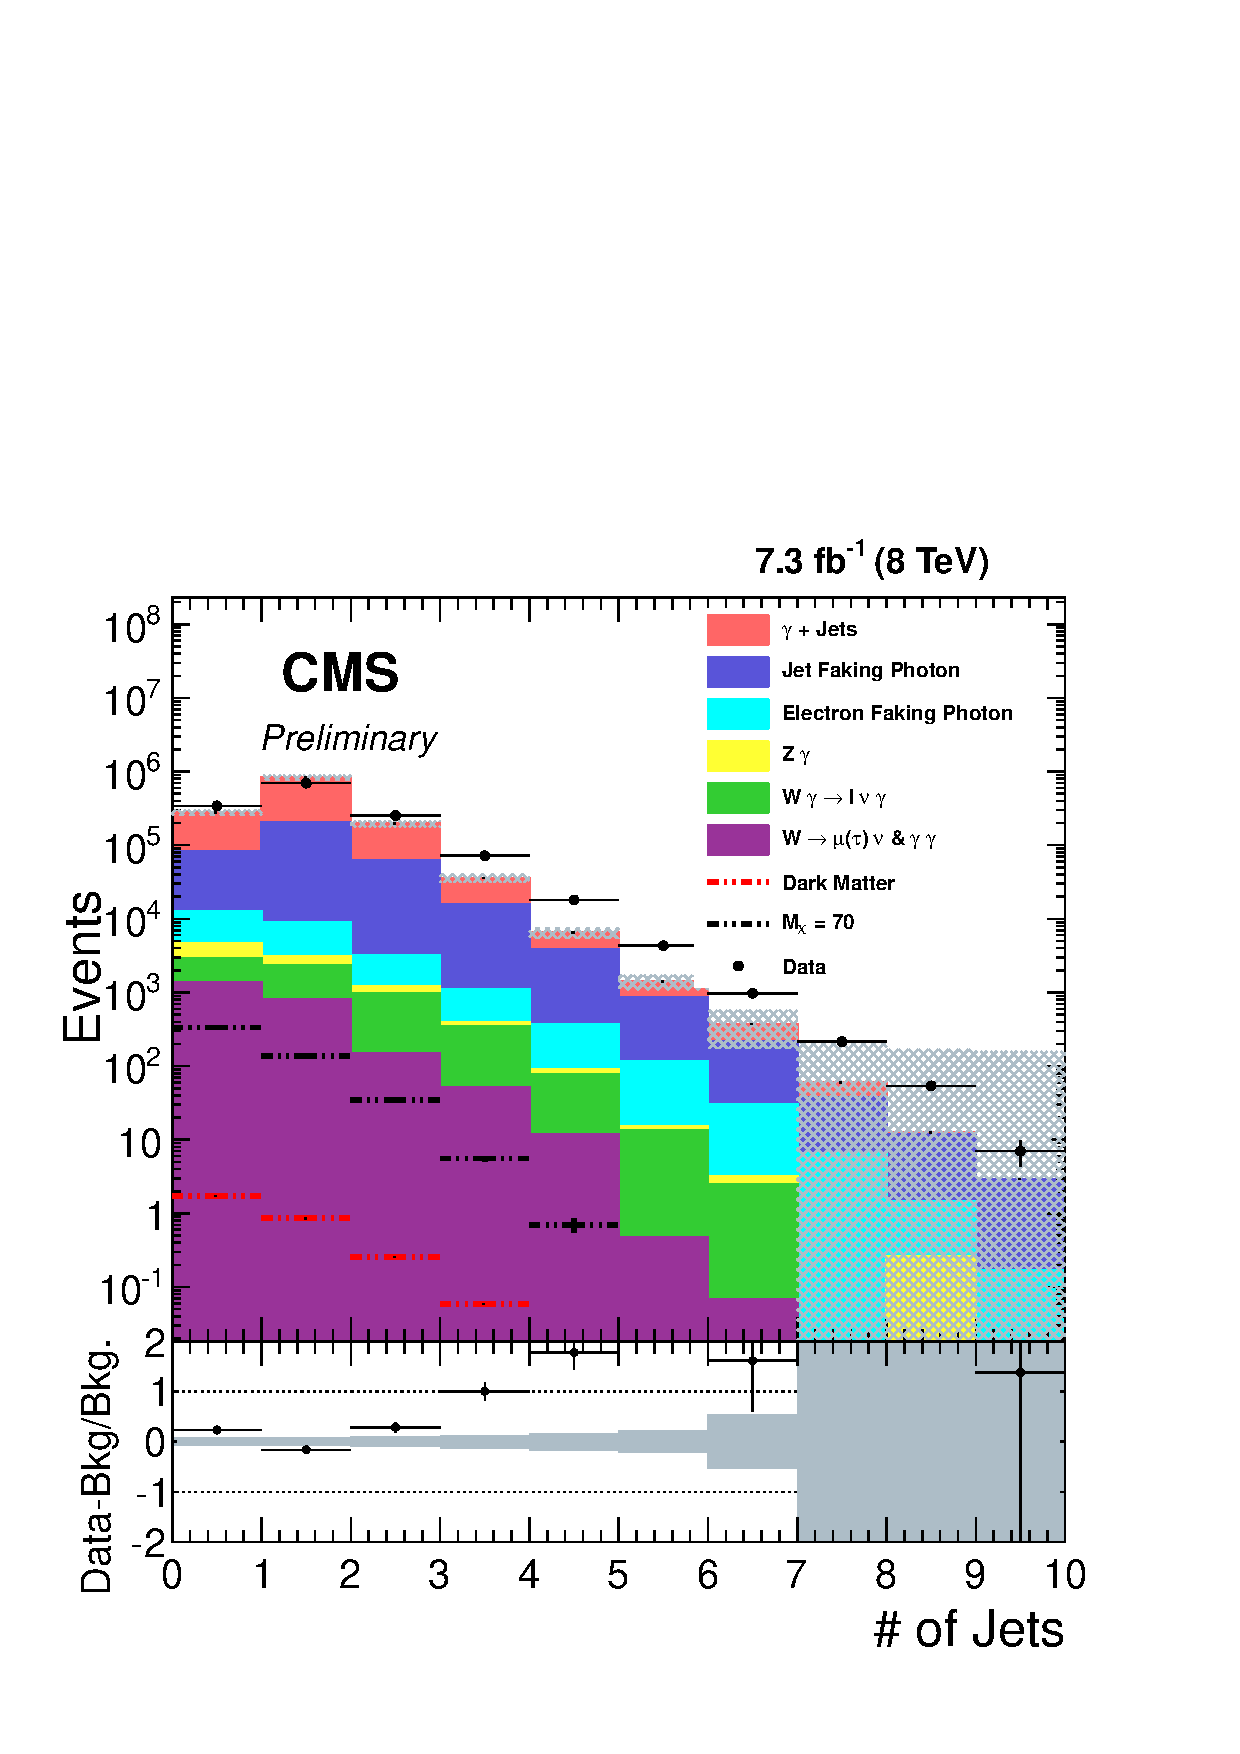
\includegraphics[width=0.45\textwidth]{analysis_figs/pythia.pdf}}
  {\label{fig:pythia}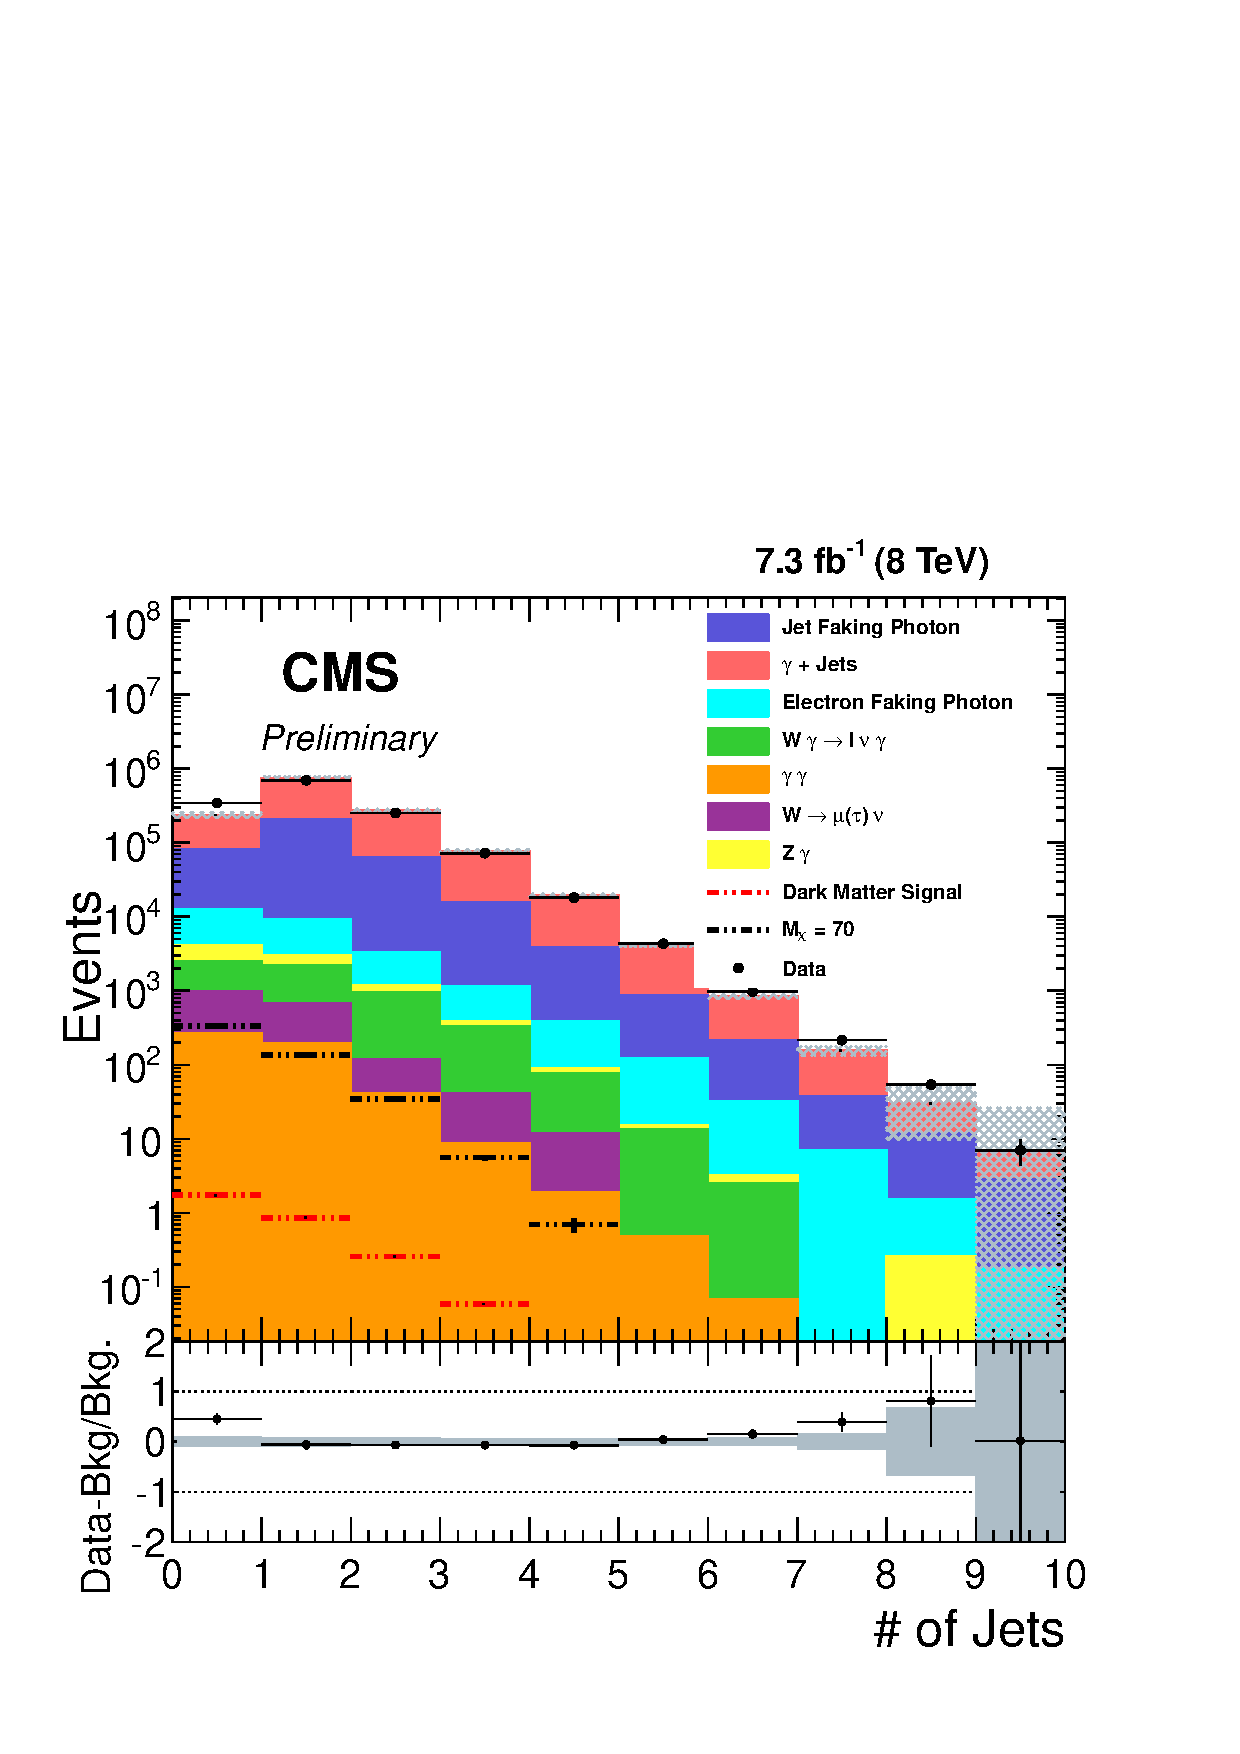
\includegraphics[width=0.45\textwidth]{analysis_figs/madgraph.pdf}} 
 \caption{Number of Jets above 30 \GeV for Pythia (left) and Madgraph (right) simulation samples}
 \label{fig:njets}
\end{figure}     

We have also observed that the discrepancy in 0 jet bin remained even with the $\gamma + \met$ madgraph sample. Therefore in conclusion we don't have a precise MC Simulation based way of estimating $\gamma + \met$ background rate. Therefore we have decided to construct a control sample where we measure the rate of this background with respect to data in different jet bins using the jet binning definitions given in Section 4.5 .

In this control sample, we have selected events triggered only by the prescaled single photon trigger. By going to a prescaled trigger, we would only have $20\%$ of the full data however, this way, we won't have any restriction on the $\met$ coming from to the trigger. To get to a region completely orthogonal to our signal selection,  we required $\met < 40.$. In this region we look at the $\gamma + jet$ production, in 2 different jet bins, by normalizing the expected yields to data after subtracting all other backgrounds from the data. The overall distributions can be seen in Fig.~\ref{fig:control_prescale1}. Based on these distributions, we have scale up the $\gamma + jet$ cross section in 0 Jet bin catagory by 1.7 and greater than 0 Jet bin catagory by 1.1. 


\begin{figure}[!h]
 \centering
  {\label{fig:madgraph}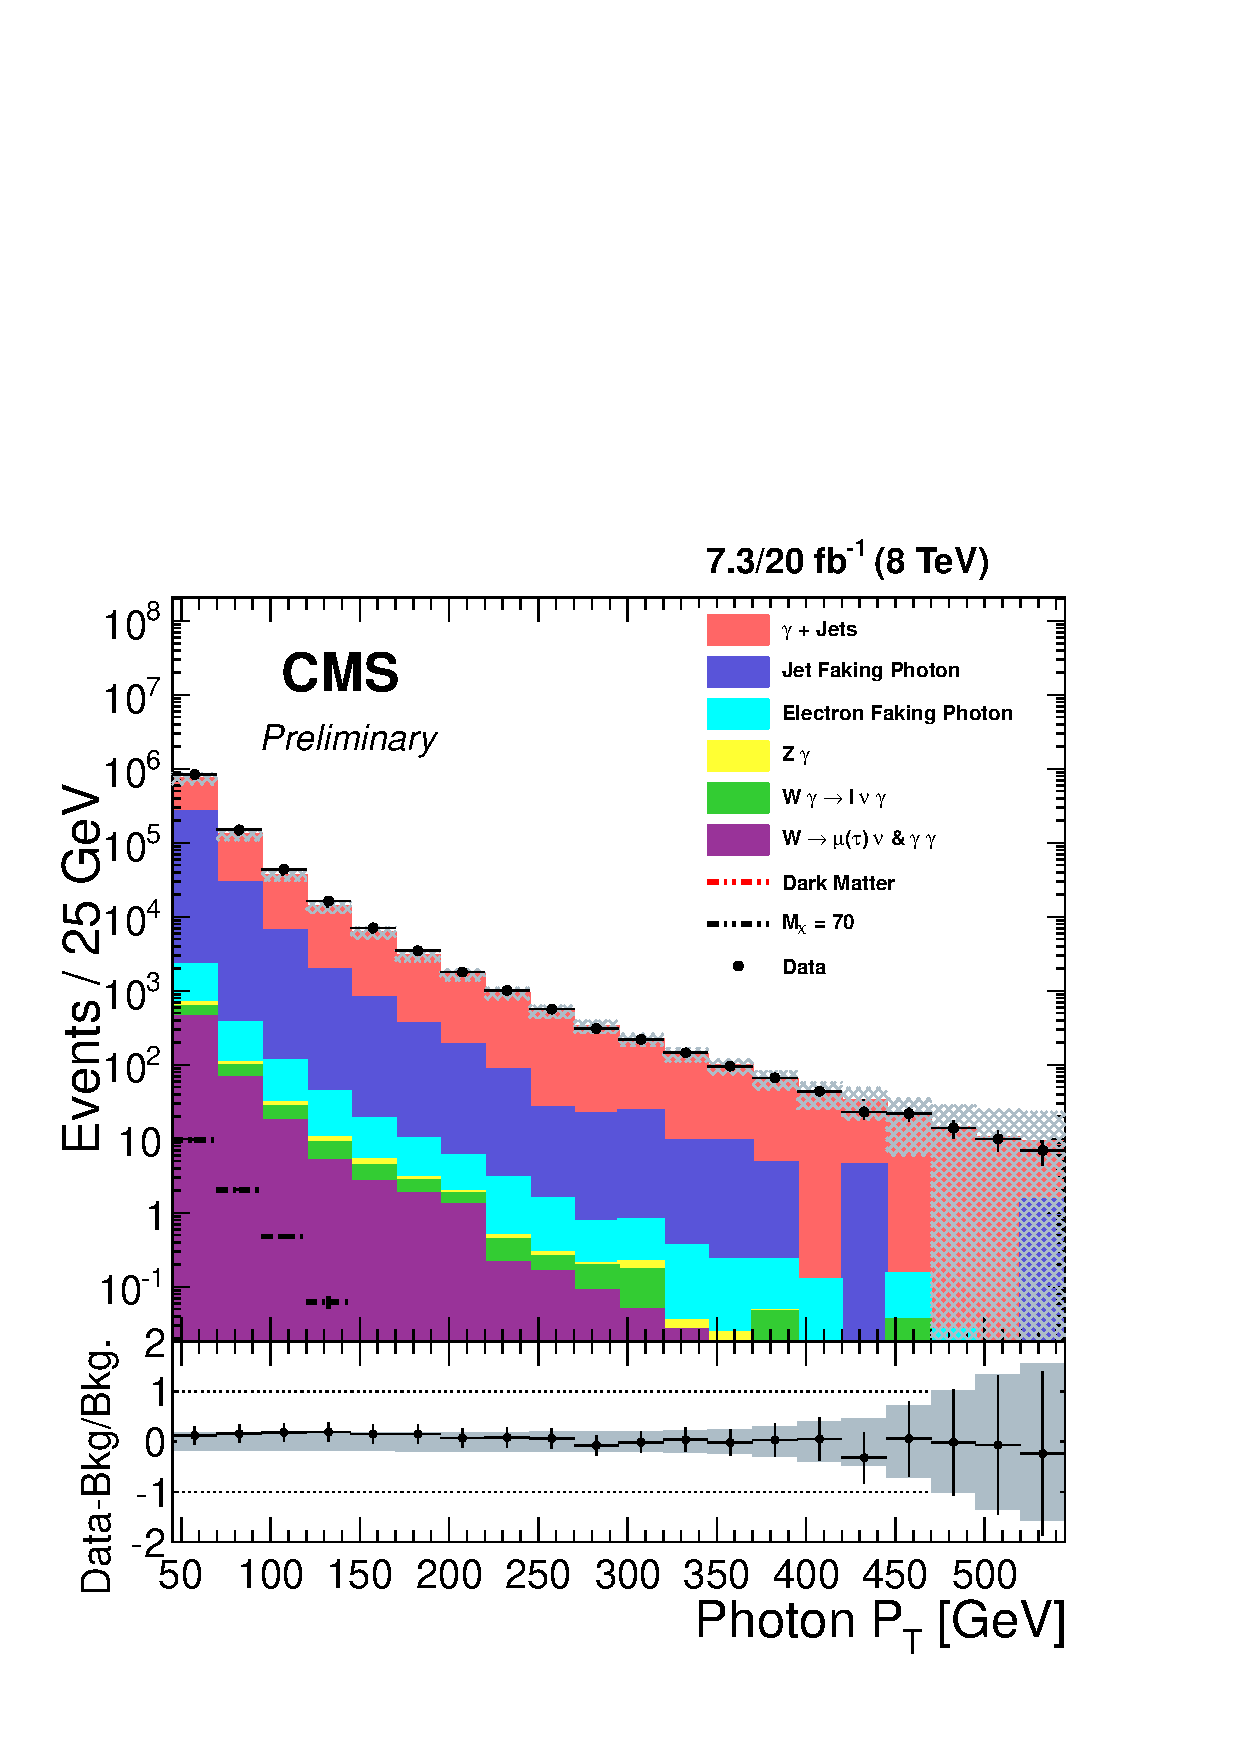
\includegraphics[width=0.45\textwidth]{analysis_figs/prescale_pt.pdf}}
  {\label{fig:pythia}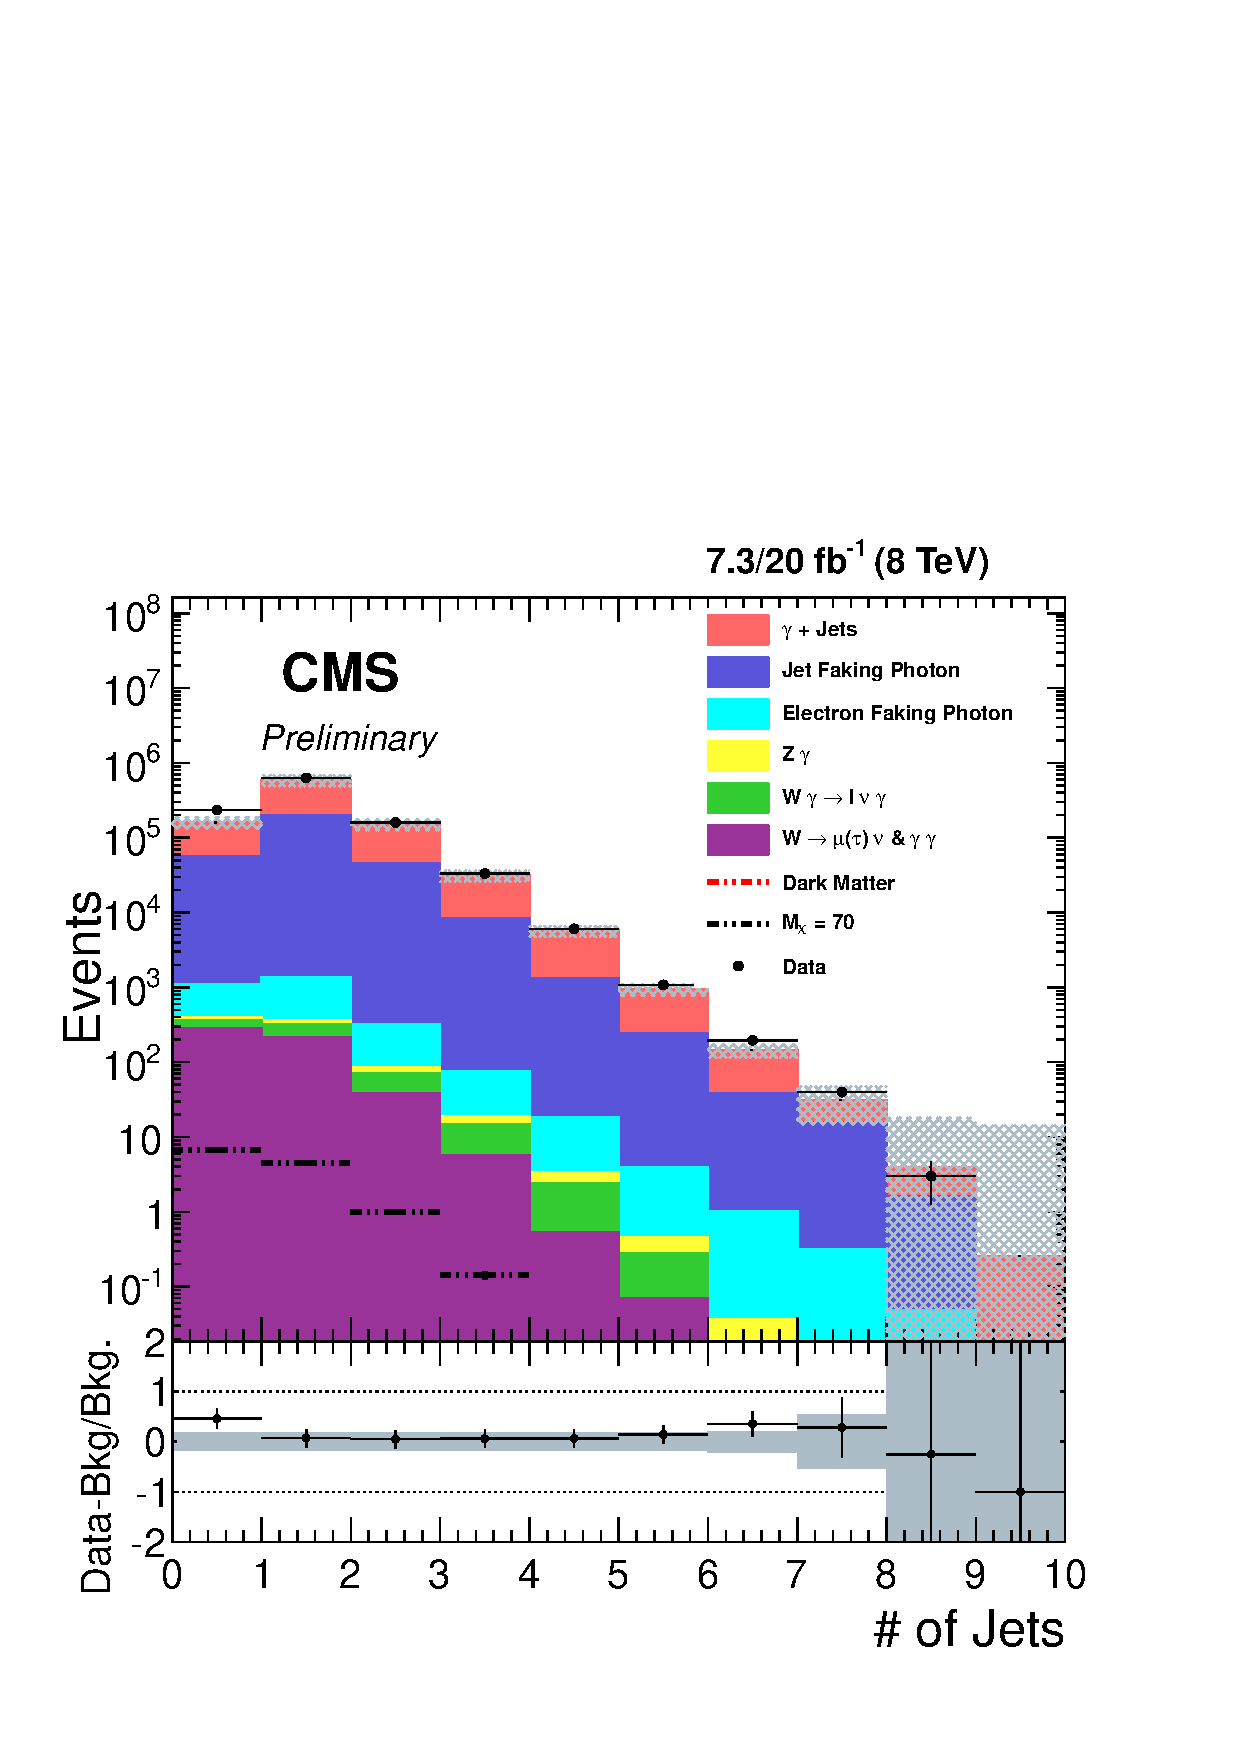
\includegraphics[width=0.45\textwidth]{analysis_figs/prescale_njet.pdf}}
 \caption{Photon Pt (left) and NJets (right) distribution for the control region. }
 \label{fig:control_prescale1}
\end{figure}

\subsection{Other MC Backgrounds}

The other MC backgrounds that we use are W$\to \mu\nu$ and W$\to \tau\nu$ and $\gamma$ + Jets. We do not apply any factors for the Wl$\nu$ backgrounds, as are significantly reduced with lepton vetos. However due to avoid overlaps with the data driven jet fake background, we have only considered the leptonic decays of W$\to \tau\nu$ background, explicitly removing the hadronic part. 
